%  A simple AAU report template.
%  2015-05-08 v. 1.2.0
%  Copyright 2010-2015 by Jesper Kjær Nielsen <jkn@es.aau.dk>
%
%  This is free software: you can redistribute it and/or modify
%  it under the terms of the GNU General Public License as published by
%  the Free Software Foundation, either version 3 of the License, or
%  (at your option) any later version.
%
%  This is distributed in the hope that it will be useful,
%  but WITHOUT ANY WARRANTY; without even the implied warranty of
%  MERCHANTABILITY or FITNESS FOR A PARTICULAR PURPOSE.  See the
%  GNU General Public License for more details.
%
%  You can find the GNU General Public License at <http://www.gnu.org/licenses/>.
%
%  A simple AAU report template.
%  2015-05-08 v. 1.2.0
%  Copyright 2010-2015 by Jesper Kjær Nielsen <jkn@es.aau.dk>
%
%  This is free software: you can redistribute it and/or modify
%  it under the terms of the GNU General Public License as published by
%  the Free Software Foundation, either version 3 of the License, or
%  (at your option) any later version.
%
%  This is distributed in the hope that it will be useful,
%  but WITHOUT ANY WARRANTY; without even the implied warranty of
%  MERCHANTABILITY or FITNESS FOR A PARTICULAR PURPOSE.  See the
%  GNU General Public License for more details.
%
%  You can find the GNU General Public License at <http://www.gnu.org/licenses/>.
%
\documentclass[12pt,twoside,a4paper,openright]{report}
%%%%%%%%%%%%%%%%%%%%%%%%%%%%%%%%%%%%%%%%%%%%%%%%
% Language, Encoding and Fonts
% http://en.wikibooks.org/wiki/LaTeX/Internationalization
%%%%%%%%%%%%%%%%%%%%%%%%%%%%%%%%%%%%%%%%%%%%%%%%
% Select encoding of your inputs. Depends on
% your operating system and its default input
% encoding. Typically, you should use
%   Linux  : utf8 (most modern Linux distributions)
%            latin1 
%   Windows: ansinew
%            latin1 (works in most cases)
%   Mac    : applemac
% Notice that you can manually change the input
% encoding of your files by selecting "save as"
% an select the desired input encoding. 
\usepackage[utf8]{inputenc}
% Make latex understand and use the typographic
% rules of the language used in the document.
\usepackage[danish,english]{babel}
% Use the palatino font
\usepackage[sc]{mathpazo}
\linespread{1.05}         % Palatino needs more leading (space between lines)
% Choose the font encoding
\usepackage[T1]{fontenc}
%%%%%%%%%%%%%%%%%%%%%%%%%%%%%%%%%%%%%%%%%%%%%%%%
% Graphics and Tables
% http://en.wikibooks.org/wiki/LaTeX/Importing_Graphics
% http://en.wikibooks.org/wiki/LaTeX/Tables
% http://en.wikibooks.org/wiki/LaTeX/Colors
%%%%%%%%%%%%%%%%%%%%%%%%%%%%%%%%%%%%%%%%%%%%%%%%
% load a colour package
\usepackage{xcolor}
\definecolor{aaublue}{RGB}{33,26,82}% dark blue
% The standard graphics inclusion package
\usepackage{graphicx}
% Set up how figure and table captions are displayed
\usepackage{caption}
\captionsetup{%
  font=footnotesize,% set font size to footnotesize
  labelfont=bf % bold label (e.g., Figure 3.2) font
}
% Make the standard latex tables look so much better
\usepackage{array,booktabs}
% Enable the use of frames around, e.g., theorems
% The framed package is used in the example environment
\usepackage{framed}

%%%%%%%%%%%%%%%%%%%%%%%%%%%%%%%%%%%%%%%%%%%%%%%%
% Mathematics
% http://en.wikibooks.org/wiki/LaTeX/Mathematics
%%%%%%%%%%%%%%%%%%%%%%%%%%%%%%%%%%%%%%%%%%%%%%%%
% Defines new environments such as equation,
% align and split 
\usepackage{amsmath}
% Adds new math symbols
\usepackage{amssymb}
% Use theorems in your document
% The ntheorem package is also used for the example environment
% When using thmmarks, amsmath must be an option as well. Otherwise \eqref doesn't work anymore.
\usepackage[framed,amsmath,thmmarks]{ntheorem}

%%%%%%%%%%%%%%%%%%%%%%%%%%%%%%%%%%%%%%%%%%%%%%%%
% Page Layout
% http://en.wikibooks.org/wiki/LaTeX/Page_Layout
%%%%%%%%%%%%%%%%%%%%%%%%%%%%%%%%%%%%%%%%%%%%%%%%
% Change margins, papersize, etc of the document
\usepackage[
  inner=28mm,% left margin on an odd page
  outer=41mm,% right margin on an odd page
  ]{geometry}
% Modify how \chapter, \section, etc. look
% The titlesec package is very configureable
\usepackage{titlesec}
\titleformat{\chapter}
{\filcenter\normalfont\Large\bfseries}
{\chaptertitlename~\thechapter} {0.5em} {}
\titleformat*{\section}{\normalfont\Large\bfseries}
\titleformat*{\subsection}{\normalfont\large\bfseries}
\titleformat*{\subsubsection}{\normalfont\normalsize\bfseries}
%\titleformat*{\paragraph}{\normalfont\normalsize\bfseries}
%\titleformat*{\subparagraph}{\normalfont\normalsize\bfseries}

% Clear empty pages between chapters
\let\origdoublepage\cleardoublepage
\newcommand{\clearemptydoublepage}{%
  \clearpage
  {\pagestyle{empty}\origdoublepage}%
}
\let\cleardoublepage\clearemptydoublepage

% Change the headers and footers
\usepackage{fancyhdr}
\pagestyle{fancy}
\fancyhf{} %delete everything
\renewcommand{\headrulewidth}{0pt} %remove the horizontal line in the header
\fancyhead[RE]{\small\nouppercase\leftmark} %even page - chapter title
\fancyhead[LO]{\small\nouppercase\rightmark} %uneven page - section title
\fancyhead[LE,RO]{\thepage} %page number on all pages
% Do not stretch the content of a page. Instead,
% insert white space at the bottom of the page
\raggedbottom
% Enable arithmetics with length. Useful when
% typesetting the layout.
\usepackage{calc}

%%%%%%%%%%%%%%%%%%%%%%%%%%%%%%%%%%%%%%%%%%%%%%%%
% Bibliography
% http://en.wikibooks.org/wiki/LaTeX/Bibliography_Management
%%%%%%%%%%%%%%%%%%%%%%%%%%%%%%%%%%%%%%%%%%%%%%%%
\usepackage[backend=bibtex,
  bibencoding=utf8
  ]{biblatex}
\addbibresource{bib/mybib}

%%%%%%%%%%%%%%%%%%%%%%%%%%%%%%%%%%%%%%%%%%%%%%%%
% Misc
%%%%%%%%%%%%%%%%%%%%%%%%%%%%%%%%%%%%%%%%%%%%%%%%
% Add bibliography and index to the table of
% contents
\usepackage[nottoc]{tocbibind}
% Add the command \pageref{LastPage} which refers to the
% page number of the last page
\usepackage{lastpage}
% Add todo notes in the margin of the document
\usepackage[
%  disable, %turn off todonotes
  colorinlistoftodos, %enable a coloured square in the list of todos
  textwidth=\marginparwidth, %set the width of the todonotes
  textsize=scriptsize, %size of the text in the todonotes
  ]{todonotes}

%%%%%%%%%%%%%%%%%%%%%%%%%%%%%%%%%%%%%%%%%%%%%%%%
% Hyperlinks
% http://en.wikibooks.org/wiki/LaTeX/Hyperlinks
%%%%%%%%%%%%%%%%%%%%%%%%%%%%%%%%%%%%%%%%%%%%%%%%
% Enable hyperlinks and insert info into the pdf
% file. Hypperref should be loaded as one of the 
% last packages
\usepackage{hyperref}
\hypersetup{%
	pdfpagelabels=true,%
	plainpages=false,%
	pdfauthor={Author(s)},%
	pdftitle={Title},%
	pdfsubject={Subject},%
	bookmarksnumbered=true,%
	colorlinks=false,%
	citecolor=black,%
	filecolor=black,%
	linkcolor=black,% you should probably change this to black before printing
	urlcolor=black,%
	pdfstartview=FitH%
}% package inclusion and set up of the document
% see, e.g., http://en.wikibooks.org/wiki/LaTeX/Formatting#Hyphenation
% for more information on word hyphenation
\hyphenation{ex-am-ple hy-phen-a-tion short}
\hyphenation{long la-tex}
% 
%  A simple AAU report template.
%  2015-05-08 v. 1.2.0
%  Copyright 2010-2015 by Jesper Kjær Nielsen <jkn@es.aau.dk>
%
%  This is free software: you can redistribute it and/or modify
%  it under the terms of the GNU General Public License as published by
%  the Free Software Foundation, either version 3 of the License, or
%  (at your option) any later version.
%
%  This is distributed in the hope that it will be useful,
%  but WITHOUT ANY WARRANTY; without even the implied warranty of
%  MERCHANTABILITY or FITNESS FOR A PARTICULAR PURPOSE.  See the
%  GNU General Public License for more details.
%
%  You can find the GNU General Public License at <http://www.gnu.org/licenses/>.
%
%
%
% see, e.g., http://en.wikibooks.org/wiki/LaTeX/Customizing_LaTeX#New_commands
% for more information on how to create macros

%%%%%%%%%%%%%%%%%%%%%%%%%%%%%%%%%%%%%%%%%%%%%%%%
% Macros for the titlepage
%%%%%%%%%%%%%%%%%%%%%%%%%%%%%%%%%%%%%%%%%%%%%%%%
%Creates the aau titlepage
\newcommand{\aautitlepage}[3]{%
  {
    %set up various length
    \ifx\titlepageleftcolumnwidth\undefined
      \newlength{\titlepageleftcolumnwidth}
      \newlength{\titlepagerightcolumnwidth}
    \fi
    \setlength{\titlepageleftcolumnwidth}{0.5\textwidth-\tabcolsep}
    \setlength{\titlepagerightcolumnwidth}{\textwidth-2\tabcolsep-\titlepageleftcolumnwidth}
    %create title page
    \thispagestyle{empty}
    \noindent%
    \begin{tabular}{@{}ll@{}}
      \parbox{\titlepageleftcolumnwidth}{
        \iflanguage{danish}{%
          
\includegraphics[width=\titlepageleftcolumnwidth]{figures/aau_logo_da}
        }{%
          
\includegraphics[width=\titlepageleftcolumnwidth]{figures/aau_logo_en}
        }
      } &
      \parbox{\titlepagerightcolumnwidth}{\raggedleft\sf\small
        #2
      }\bigskip\\
       #1 &
      \parbox[t]{\titlepagerightcolumnwidth}{%
      \textbf{Abstract:}\bigskip\par
        \fbox{\parbox{\titlepagerightcolumnwidth-2\fboxsep-2\fboxrule}{%
          #3
        }}
      }\\
    \end{tabular}
    \vfill
    \iflanguage{danish}{%
      \noindent{\footnotesize\emph{Rapportens indhold er frit tilgængeligt, men offentliggørelse (med kildeangivelse) må kun ske efter aftale med forfatterne.}}
    }{%
      \noindent{\footnotesize\emph{The content of this report is freely available, but publication (with reference) may only be pursued due to agreement with the author.}}
    }
    \clearpage
  }
}

%Create english project info
\newcommand{\englishprojectinfo}[8]{%
  \parbox[t]{\titlepageleftcolumnwidth}{
    \textbf{Title:}\\ #1\bigskip\par
    \textbf{Theme:}\\ #2\bigskip\par
    \textbf{Project Period:}\\ #3\bigskip\par
    \textbf{Project Group:} #4\bigskip\par
    \textbf{Participant(s):}\\ #5\bigskip\par
    \textbf{Supervisor(s):}\\ #6\bigskip\par
    \textbf{Copies:} #7\bigskip\par
    \textbf{Page Numbers:} \pageref{LastPage}\bigskip\par
    \textbf{Date of Completion:}\\ #8
  }
}

%Create danish project info
\newcommand{\danishprojectinfo}[8]{%
  \parbox[t]{\titlepageleftcolumnwidth}{
    \textbf{Titel:}\\ #1\bigskip\par
    \textbf{Tema:}\\ #2\bigskip\par
    \textbf{Projektperiode:}\\ #3\bigskip\par
    \textbf{Projektgruppe:}\\ #4\bigskip\par
    \textbf{Deltager(e):}\\ #5\bigskip\par
    \textbf{Vejleder(e):}\\ #6\bigskip\par
    \textbf{Oplagstal:} #7\bigskip\par
    \textbf{Sidetal:} \pageref{LastPage}\bigskip\par
    \textbf{Afleveringsdato:}\\ #8
  }
}

%%%%%%%%%%%%%%%%%%%%%%%%%%%%%%%%%%%%%%%%%%%%%%%%
% An example environment
%%%%%%%%%%%%%%%%%%%%%%%%%%%%%%%%%%%%%%%%%%%%%%%%
\theoremheaderfont{\normalfont\bfseries}
\theorembodyfont{\normalfont}
\theoremstyle{break}
\def\theoremframecommand{{\color{gray!50}\vrule width 5pt \hspace{5pt}}}
\newshadedtheorem{exa}{Example}[chapter]
\newenvironment{example}[1]{%
		\begin{exa}[#1]
}{%
		\end{exa}
}

%%%%%%%%%%%%%%%%%%%%%%%%%%
% Macros for refenencing %
%%%%%%%%%%%%%%%%%%%%%%%%%%
\newcommand{\figref}[1]{Figure \ref{#1}}
\newcommand{\tabref}[1]{Table \ref{#1}}
\newcommand{\secref}[1]{Section \ref{#1}}
\newcommand{\chapref}[1]{Chapter \ref{#1}}
\newcommand{\coderef}[1]{Listing \ref{#1}}
\newcommand{\appref}[1]{Appendix \ref{#1}}% my new macros

\begin{document}
%frontmatterf
\pagestyle{empty} %disable ers and footers
\pagenumbering{roman} %use roman page numbering in the frontmatter
%  A simple AAU report template.
%  2015-05-08 v. 1.2.0
%  Copyright 2010-2015 by Jesper Kjær Nielsen <jkn@es.aau.dk>
%
%  This is free software: you can redistribute it and/or modify
%  it under the terms of the GNU General Public License as published by
%  the Free Software Foundation, either version 3 of the License, or
%  (at your option) any later version.
%
%  This is distributed in the hope that it will be useful,
%  but WITHOUT ANY WARRANTY; without even the implied warranty of
%  MERCHANTABILITY or FITNESS FOR A PARTICULAR PURPOSE.  See the
%  GNU General Public License for more details.
%
%  You can find the GNU General Public License at <http://www.gnu.org/licenses/>.
%
\pdfbookmark[0]{Front page}{label:frontpage}%
\begin{titlepage}
  \addtolength{\hoffset}{0.5\evensidemargin-0.5\oddsidemargin} %set equal margins on the frontpage - remove this line if you want default margins
  \noindent%
  \begin{tabular}{@{}p{\textwidth}@{}}
    \toprule[2pt]
    \midrule
    \vspace{0.2cm}
    \begin{center}
    \Huge{\textbf{
      Less obstructed street traffic% insert your title here
    }}
    \end{center}
    \begin{center}
      \Large{
        - Subtitle -% insert your subtitle here
      }
    \end{center}
    \vspace{0.2cm}\\
    \midrule
    \toprule[2pt]
  \end{tabular}
  \vspace{4 cm}
  \begin{center}
    {\large
      Project Report%Insert document type (e.g., Project Report)
    }\\
    \vspace{0.2cm}
    {\Large
      D505E15%Insert your group name or real names here
    }
  \end{center}
  \vfill
  \begin{center}
  Aalborg University\\
  Electronics and IT
  \end{center}
\end{titlepage}
\clearpage

\thispagestyle{empty}
{\small
\strut\vfill % push the content to the bottom of the page
\noindent Copyright \copyright{} Aalborg University 2015\par
\vspace{0.2cm}
\noindent Here you can write something about which tools and software you have used for typesetting the document, running simulations and creating figures. If you do not know what to write, either leave this page blank or have a look at the colophon in some of your books.
}
\clearpage


\pdfbookmark[0]{English title page}{label:titlepage_en}
\aautitlepage{%
  \englishprojectinfo{
    Less Obstructed Street Traffic%title
  }{%
    Intelligent or Massively Parallel Systems %theme
  }{%
    Fall Semester 2015 %project period
  }{%
    d505e15 % project group
  }{%
    %list of group members
    Andreas Hairing Klostergaard\\
    Benjamin Ahm\\
    Kristian Hauge Jensen\\
    Michael Jensen\\
    Morten Rune Petersen\\
    Morten Korsholm Terndrup
  }{%
    %list of supervisors
    Bin Yang
  }{%
    2 % number of printed copies
  }{%
    \today % date of completion
  }%
}{%department and address
  \textbf{Department of Computer Science}\\
  Aalborg University\\
  Selma Lagerlöfsvej 300\\
  9000 Aalborg\\
  \href{http://www.aau.dk}{http://www.aau.dk}
}{% the abstract
This report addresses the problem of traffic congestion by proposing an approach for finding traffic patterns using Machine Intelligence techniques supported by a distributed system used to gather data. The report considers an regression approach to predict future traffic speeds based on previously observed speeds on roads. A system utilizing the regression models as weights in a directed graph of a road network to find routes is constructed. The system aims to find routes that maximize time savings for users by accurately modeling the traffic through the regression models. The accuracy of the models is evaluated and the system is shown to potentially alleviate congestion.}

\cleardoublepage
%{\selectlanguage{danish}
%\pdfbookmark[0]{Danish title page}{label:titlepage_da}
%\aautitlepage{%
%  \danishprojectinfo{
%    Rapportens titel %title
%  }{%
%    Semestertema %theme
%  }{%
%    Efterårssemestret 2010 %project period
%  }{%
%    XXX % project group
%  }{%
%    %list of group members
%    Forfatter 1\\
%    Forfatter 2\\
%    Forfatter 3
%  }{%
%    %list of supervisors
%    Vejleder 1\\
%    Vejleder 2
%  }{%
%    1 % number of printed copies
%  }{%
%    \today % date of completion
%  }%
%}{%department and address
%  \textbf{Elektronik og IT}\\
%  Aalborg Universitet\\
%  \href{http://www.aau.dk}{http://www.aau.dk}
%}{% the abstract
%  Her er resuméet
%}}

\cleardoublepage
\pdfbookmark[0]{Contents}{label:contents}
\pagestyle{fancy} %enable headers and footers again
\tableofcontents
\listoftodos
\chapter*{Preface\markboth{Preface}{Preface}}\label{ch:preface}
\addcontentsline{toc}{chapter}{Preface}
This report is part of a 5th semester project as a part of the semester courses at Aalborg University. The point of the project is to achieve a set of learning goals specified by the study regulation for Computer Science bachelors degree. More specifically, the goal is to achieve knowledge, skills and competencies within the fields of Machine Intelligence, which is the primary focus of this project.
Since not all project group members are following the optional machine intelligence course, machine learning techniques are supported by Distributed Systems and Network techniques. The reason for this is to also achieve knowledge, skills and competencies about this field as well since this is naturally important for some of the group members.
We believe we have achieved the goals of the study regulation through the work documented in the report. We have achieved knowledge, skills and competencies about different machine learning techniques through the analysis, implementation and evaluation of the techniques for learning traffic patterns. 
We would like to extend our thanks to Fabrice Marchal and TrackMatching for being helpful and providing increased quotes for their excellent service.

\vspace{\baselineskip}\hfill Aalborg University, \today
\vfill\noindent
\begin{minipage}[b]{0.45\textwidth}
 \centering
 \rule{\textwidth}{0.5pt}\\
  Andreas Hairing Klostergaard\\
 {\footnotesize <aklost11@student.aau.dk>}
\end{minipage}
\hfill
\begin{minipage}[b]{0.45\textwidth}
 \centering
 \rule{\textwidth}{0.5pt}\\
  Benjamin Ahm\\
 {\footnotesize <bahm13@student.aau.dk>}
\end{minipage}

\vspace{3\baselineskip}\noindent
\begin{minipage}[b]{0.45\textwidth}
 \centering
 \rule{\textwidth}{0.5pt}\\
  Kristian Hauge Jensen\\
 {\footnotesize <kje13@student.aau.dk>}
\end{minipage}
\hfill
\begin{minipage}[b]{0.45\textwidth}
 \centering
 \rule{\textwidth}{0.5pt}\\
  Michael Jensen\\
 {\footnotesize <mj09@student.aau.dk>}
\end{minipage}

\vspace{3\baselineskip}\noindent
\begin{minipage}[b]{0.45\textwidth}
 \centering
 \rule{\textwidth}{0.5pt}\\
  Morten Rune Peterson\\
 {\footnotesize <mopete13@student.aau.dk>}
\end{minipage}
\hfill
\begin{minipage}[b]{0.45\textwidth}
 \centering
 \rule{\textwidth}{0.5pt}\\
  Morten Korsholm Terndrup\\
 {\footnotesize <mternd13@student.aau.dk>}
\end{minipage}

\cleardoublepage
%mainmatter
\pagenumbering{arabic} %use arabic page numbering in the mainmatter
\chapter{Introduction}
Transportation problems arise frequently in areas with high population density. Examples that come to mind are people standing in line for services, traffic congestion on roads, and overcrowded public transportation. Many of these problems become accentuated when notable events occur, such as concerts, people going on holidays, and traffic accidents. Designing an infrastructure with these potential problems in mind can certainly minimize the troubles they cause. However, infrastructures are typically designed with a particular context in mind and consequently do not respond well to serious changes in the area, such as an increasing number of people. Costs are high when roads have to be expanded, changed, or constructed, and maintenance costs increase as roads more regularly need to be renewed when the everyday traffic in the area increases. For these reasons, it is advantageous to achieve better utilisation of road networks, such that costs of overburdened roads can be lowered as well as saving time for the people stuck in traffic congestions. This leads to an initial problem for this project: How can we analyse traffic to detect current and possibly future problems, such that initiatives for alleviating them can be considered.\todo{Læs intro. Måske nogle ting her, der tilhører relevans}
\chapter{Problem analysis}
\section{Relevance}
Traffic problems has several consequences and affects several different groups of people and organizations. Estimates show that the number of cars in the world is increasing year by year\cite{WardsAuto:CarPopulation}. This increase can potentially lead to an increase in traffic congestions, which in turn increases the need for better infrastructure or more efficient traffic flow. 
% wear on roads
Likewise, many of the roads that are congested are heavily used roads. These roads see more wear than less used roads and therefore requires either special construction or more maintenance, which increases the costs for governments on infrastructure. Maintenance of roads also obstructs the road network, since parts of a road can be unavailable which can result in temporarily slower traffic.
% Emissions
Another issue that is a consequence of traffic congestion is the increased CO2-emissions of vehicles continuously accelerating and de-accelerating in a congested area\cite{BarthBoriboonsomsin2009}.\\
% Time wasted --> stress
Being stuck in traffic can also affect the well-being of drivers as stress-levels increase. A study of the relationship between traffic congestion and driver stress observes that there is a correlation between drivers stressed behaviour and the traffic situation\cite{HennesyWiesenthal1997}\cite{StokolsNovacoStokolsCampell1978}. Stress has several negative impacts on the health of the stressed individual, which in worst case can lead to medical problems. Furthermore, severely stressed drivers can risk driving recklessly to get out of congestion, endangering themselves and others in traffic\cite{Shinar1998}. \\
% Emergency vehicles obstructed by congestion
Another critical issue is that emergency vehicles needing to travel through congested areas might be obstructed by traffic congestion. This is can at the worst case result in life-threatening situations which is why avoiding congestion is critical.
The economic consequences of traffic congestion are severe as the combined annual costs of congestion in U.S., U.K., France and Germany is estimated to increase to \$293.1 billion by 2030\cite{INRIX2013}. For		 individuals this translates into an annual, average cost of \$1740 and 111 hours wasted stuck in traffic.\\
To sum up the various issues of traffic congestion and whom they affect, \tabref{tab:relevance} shows a summary.

\begin{table}[]
\centering
\caption{Summary of issues involving interested parties}
\label{tab:relevance}
\begin{tabular}{lllll}
\multicolumn{1}{c|}{Interested party} & \multicolumn{1}{c}{Affected by}                                                                                                 &  &  &  \\ \cline{1-2}
\multicolumn{1}{l|}{Drivers}          & \begin{tabular}[c]{@{}l@{}}time wasted in traffic\\ stress from congestion\\ CO2-emissions\\ costs of congestion\end{tabular}   &  &  &  \\ \cline{1-2}
\multicolumn{1}{l|}{Governments}      & \begin{tabular}[c]{@{}l@{}}maintenance costs\\ emergency vehicle obstruction\\ CO2-emissions\\ costs of congestion\end{tabular} &  &  &  \\
                                      &                                                                                                                                 &  &  & 
\end{tabular}
\end{table}
\section{Existing work}
The simpler way of receiving updates on traffic is through the radio in your car. This method is still used to inform people if there has been some incident or if there is heavy traffic on some road. Though this is only to inform people and they usually do not suggest alternative routes to avoid the heavy traffic. The message is reported in by a person and is typically announced once. \todo{Måske skal det her op i introduction}

There exists vast ways of planning a route on different devices and there is  a lot of research in this field as well, trying to figure out ways to improve the already existing technologies and techniques. The earliest versions of simple GPS-devices, which could aid in finding a route, only considered the shortest path or the fastest path to your destination.\todo{Source?}

The recent years there has been focus on trying to predict other things like live traffic patterns and changing conditions on your route.\todo{Source?}

In the following section relevant existing technologies and scientific articles will be explored so as to gain insight into the existing work of the problem domain.
%Though it is necessary to first explain shortly what GPS is and what it does, since it is the key technology for all route planning devices.

\subsection*{Dedicated GPS products}
A typical GPS, such as a TomTom device works by using satellites. It locates your position and then locate the point you want to navigate to, then it computes a route on a map, which is usually on a SD-card inside the TomTom device. There is no historical data applied to generate the routes.

It also uses a technology called RDS-TMC (Radio Data System-Traffic Message Channel), which is a service that provides live-time traffic updates to your GPS. RDS-TMC works such that if there is an incident on a road, such as a crash, bad weather or queues it transmits data about this to a central information centre, that further transmit the information to a TMC information service provider. The information service provider encodes the traffic information, and transmits it to a FM radio broadcast where the information is then sent out in RDS signals which the GPS-device receives and decodes to a visual representation.

\subsection*{Web Mapping Services}
%GPS consists of 3 key elements, namely the satellites in space, monitoring stations on earth and a person and his GPS receiver. The satellites are needed to pinpoint a location on earth, where you need atleast 4 satellites to accomplish that. 
%There are 4 unmanned monitoring stations and one manned, the unmanned stations receive constant data from the satellites and they forward it to the manned station, which then corrects the data and afterwards sends the data back up to the satellites  again. The satellites transmits low power radio signals on different frequencies for different users.
%http://www.tomtom.com/howdoesitwork/page.php?ID=5\&CID=2\&Language=1
%The exact method to pinpoint your location with the 4 or more satellites is through trilateration. The way trilateration works is illustrated in figur(trilateration), though this is only in 2D, where in the real world it is 3D, but the point is the same except it is just spheres instead of circles.
%http://www.tomtom.com/howdoesitwork/page.php?ID=8\&CID=2\&Language=1\&Lid=4
%
Google Maps developed by Google is a Web Mapping Service that people can download to their mobile devices such as smartphones. It has a feature where the suggested routes will be coloured green, yellow or red indicating respectively clear, slow-moving or heavily congested traffic.

Google Maps creates the routes from historical data and live data which is sent by sensors and smartphones\todo{source http://www.google.com/maps/about/}. The historical data includes information about what day it is and what time of the day it is, to be able to try to predict if there can occur traffic jams. The live data which are sent by sensors are placed by the government or private companies who gather traffic information, where the live data from the smartphones are from people who are driving on the roads, reporting automatically how fast they are moving on a particular road. The map is not hardcoded on your device, but depending on your route and your whereabouts, segments of a map is downloaded to your device.


\subsection*{Intelligent Transportation Systems}
So far we have discussed the more or less chronological order of popularity of transportation systems technologies. However these devices rely on relatively simple route planning mechanisms. Now, we turn to a more advanced form of transportation system, namely the Intelligent Transportation Systems. An Intelligent Transportation System is a broad term, describing a system that provides traffic services, such that different kinds of users can better utilize transportation networks\todo{Mere eller mindre selvskreven definition, måske anvend definition fra ITS handbook}. This implies, that ITS are not necessarily 'intelligent', as to act and make decisions for the users, but can be more of a tool for users to assist in making smart choices.

\subsubsection*{Obtaining traffic data}
Any ITS must consider some data if it is to be of any real use for the user. Obtaining data is therefore one of the aspects of such a system. We distinguish between two methods of obtaining traffic data: road-based and vehicle-based data collection. 

Road-based methods places the responsibility of collection data on equipment installed on the roads, such that passing vehicles has no involvement in the collection. Road-based methods\cite{PIARC0} include technologies such as inductive loops buried beneath the roads to sense passing vehicles, and infra-red or ultrasonic sensors mounted on different entities along the roads. Inductive loops has the advantage of working well, regardless of the surrounding environment, however they are costly to implement and maintain in existing road networks, since they need to be buried beneath the roads. The sensors has the advantage of being less costly in implementation and maintenance, but may have problems operating under bad environment conditions such as snowy weather\cite{KamranHaas2007,PIARC0}.

The vehicle-based methods of collecting traffic data includes the vehicles in the responsibility of data collection. This means that vehicles might be equipped with devices that, either coorporates with some service or other equipment installed on the roads. Vehicle based methods include cell-tower triangulation of mobile devices, RFID-based identification of vehicles with sensors on the roads (or other vehicles in a peer-2-peer network) and GPS-enabled devices, communicating with a GPS service provider or satellite. Regardless of using a road-based or vehicle-based method, installing and maintaining equipment on roads for an ITS is expensive[1]. Considering the GPS-enabled devices approach is independent of other physical equipment installed in the area or on the roads, and the widespread popularity of GPS-enabled devices such as smart-phones, this approach seems like the most flexible and cost-efficient way of collecting traffic data.
% maybe- Mesh network of cars\todo{Cite Morten's source}

\subsubsection*{Analysing traffic data}
When data i readily available for an ITS, the system must perform some kind of analysis to discover useful information about transportation networks. Expecially, we are interested in the detection of road incidents such as car accidents and roadwork, and traffic congestion. Such abnormal events on a road network, can be defined as negative deviation from normal traffic flow on a given road. The normal traffic flow can be determined by collecting and processing historical data such as the speed of vehicles travelling on the road.


Someone\todo{insert source} proposes to partition road networks into road segments, such that information relevant for each segment is linked with the respective segment. This accommodates special cases of roads, such as highways, where some traffic data collected from the road is not necessarily relevant for some other part of the highway. An example would be the E45 highway, where the traffic on E45 in Northern Jylland might not be relevant for the traffic on E45 in Southern Jylland.
How can traffic data be analysed?
- Traffic states
- Road segmentation, city segmentation
- Statistical data about road segments 
\section{Current limitations}
Hvad har dette eksisterende arbejde opnåaet og ikke opnået?
\section{Method}
This section describes how we accomplish the different parts of the project. We describe our source of GPS data and how we are going to collect live data from the distributed network of GPS-devices. Furthermore we describe our mathematical model of the problem domain as well as the problem representation.

\subsection*{Data source \& collection}
For the project we will be using a GPS data set from Beijing from 10.000 taxies over a period of a week, as our historical data. A problem regarding this data is the short time span, since it does not cover holidays, or other special days, which are often at fault for massive traffical problems. We are also going to use a large data set from Beijing to simulate real-time data, this data was gathered over a period of 5 years, and include a testbase of 182 people.
Where did we get our data, and how are we going to collect (live) data?

\subsection*{Problem domain and representation}
% problem domain: what we need to know about
The problem domain is a network of roads, intersections and vehicles. One straightforward method for modelling the problem domain is as a weighted, directed graph. Let G be a graph $G(N,E)$ where $E$ is the set of edges corresponding to road segments between intersections, $N$ is the set of nodes corresponding to intersections of roads. Each edge $e_i \in E$ has an associated cost, $c(e_i)$ where  $c: E \rightarrow \mathbb Z_+^*$ is the cost function. The cost of each edge describes the preference of taking the particular road corresponding to the edge. We want to design an algorithm for the cost function, that dynamically change the cost for each edge, as the flow of traffic in the road network changes, such that better routes dynamically can be determined based on the current traffic situation.

% problem representation: driver of vehicles origin and destination. Evt. time constraints?

\section{Solution criteria}
We have chosen that the main criteria the routes generated by our solution, are to be evaluated up against, are a similar route generated by Google maps. And thereby examine whever we are generating a better route based on the traffic patterns that we have identified from the historical data. This means that we should be succesfull in navigating people arround possible traffic congestions, and other slow moving traffic. 

\textit{A hard criteria for our solution is that it has to get the vehicle from it's source start address to it's destination address, using the existing road network, and it has to comply to the restrictions that the roads have.}

Besides that it is possible to look at some of the following criteria:
\begin{itemize}
	\item Is the average speed on the normal congested road improved
	\item Is the cars using the navigation getting to their destination in a optimal way, not having to drive a massive detour,
	\item Is the traffic distributed in a good manner over the whole road network
	\item Is the time spent in congestions reduced
\end{itemize}
\clearpage
\section{Problem formulation}
So far we have considered different aspects of the abstract problem of detecting traffic patterns. However, before we construct a solution, the problem should be well-defined such that a solution is clear. The problem is defined by the following problem formulation:
\\\\
\emph{Can an intelligent agent model the road network of Beijing to process and analyse raw GPS data, collected from a network of GPS-enabled vehicles, so as to detect traffic patterns indicating abnormal traffic flow such that a map of the traffic state of a road network can be constructed, that can be used to suggest alternative routes for drivers to avoid congestion and consequently save time and in general obtain better utilization of the road network?}
\\\\
Decomposing the problem formulation, we get the following questions:

\begin{itemize}
\item How can a road network and traffic be modelled?
\item How can data be collected and communicated between GPS-devices and the agent?
\item How can the agent analyse traffic data to detect traffic patterns?
\item Can such a system deliver time savings for drivers?
\item Can such a system deliver better utilisation of road networks?
\end{itemize}

With the problem formulation defined we can now construct a solution that answers the above questions, consequently answering the problem formulation itself.

% Prob1: Can traffic patterns be identified by analysing live as well as historical GPS-data of moving vehicles, giving a more understandable picture of the traffic situation, such that road networks can be better utilised?

% input: Raw GPS data from gps devices in vehicles
% problem domain model: directed weighted graph
% problem solution model: search / constraint satisfaction problem? Search problem?
% output: "Map" of traffic incidents and congestion, where road weights have changed according to these problems
% 
\chapter{Solution (mangler bedre kapitelnavn)}
\section{Problem representation}
Before a solution for the problem formulation can be designed, the problem domain must be more precisely defined, so it is clear what the system needs to know about, and consequently a model for representing the problem can be proposed. This section describes the problem domain and a fitting model of the problem domain.

\subsection*{Domain}
\figref{fig:problem-domain} illustrates the problem domain. 
\begin{figure}[h!]
  \centering
    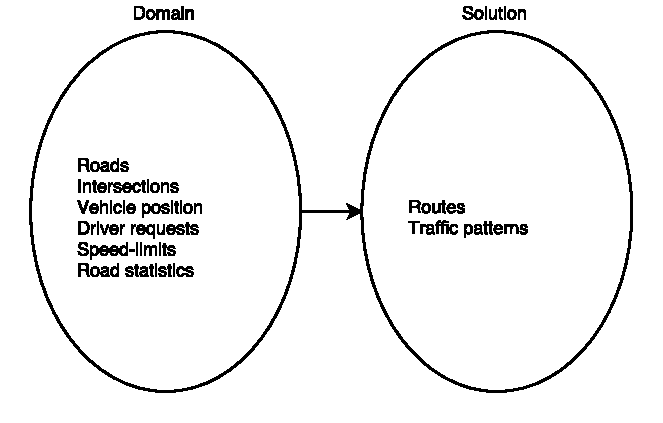
\includegraphics[width=0.8\textwidth]{figures/pd.pdf}
    \caption{Problem domain}
    \label{fig:problem-domain}
\end{figure}
\todo{Discuss and review this figure}
The problem domain consists of roads, intersections and vehicle positions a road network as well as the requirements of drivers of vehicles. The roads also include properties of said roads, such as the traffic, speed-limits and other relevant statistics about the road network. Most of these properties can be inferred from the traffic history of a given e.g. the usual speed of vehicles on that road.\todo{review the wording of the section}

\subsection*{Model}
To represent the problem domain we model the problem as a weighted, directed graph. \\
Let G be a weighted directed graph $G(N,E)$ where $E$ is the set of edges corresponding to roads between intersections and $N$ is the set of nodes corresponding to intersections of roads. Each edge $e_i \in E$ is a tuple $(n_o, n_t)$ where $n_o, n_t \in N$ and represents the direction of an edge from the origin node, $n_o$ to the target node $n_t$. Each edge also has an associated cost, $c(e_i)$ where  $c: E \rightarrow \mathbb R_+^*$ is the cost function. The cost of each edge describes the preference of taking the particular road corresponding to the edge. 

We want to design an algorithm for the cost function, that dynamically change the cost for each edge, as the flow of traffic in the road network changes, such that better routes dynamically can be determined based on the current traffic situation.\todo{discuss describing the cost function here versus other place}

\subsection*{Constraints(?)}
Here we define the constraints on the model from the problemformulation.
% problem domain --> model --> solution properties
%\section{Solution design (i mangel af bedre navn}
%This section describes the design of the system as it is implemented. First, system architecture will be presented as to gain an overview of how the system works on a high level. Then the communication between modules will be discussed, following a description of data preprocessing and analysis. At last we discuss how the route planning module of the system works.
\section{System architecture}
The design in \figref{fig:systemoverview} shows the overview of the system. 

\begin{figure}[h!]
  \centering
    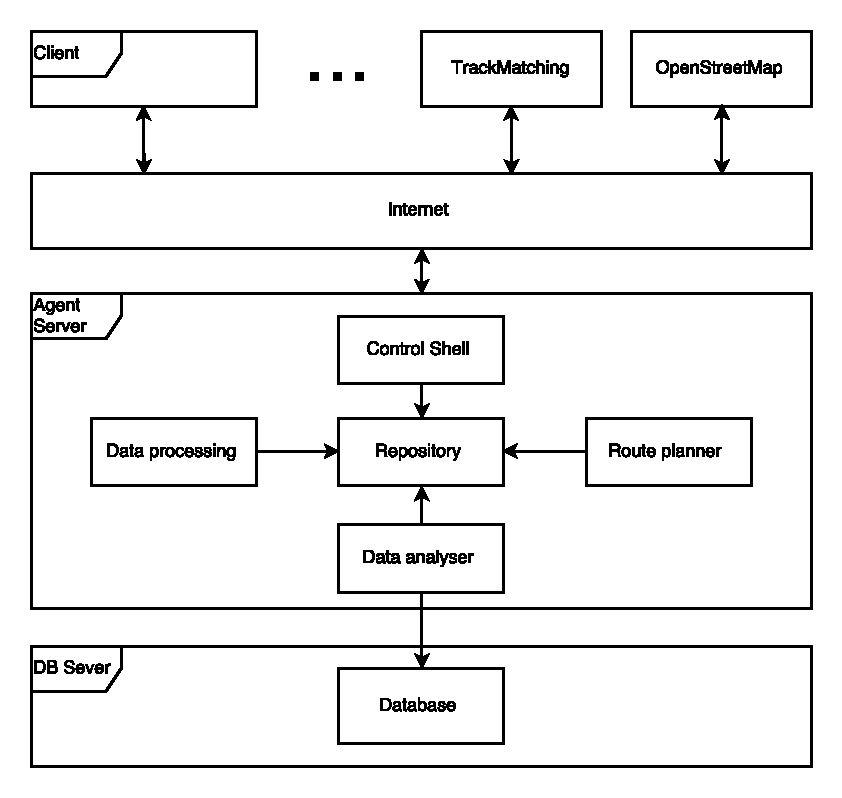
\includegraphics[width=1\textwidth]{figures/architecture.pdf}
    \caption{A course grained system overview.}
    \label{fig:systemoverview}
\end{figure}

The system has been designed as a combination of a client-server and a repository "blackboard" pattern. The main server module encapsulates most of the processing of the system. The clients represent the GPS-enabled devices that communicates live GPS data through an internet connection to the server, which in turn processes and analyses the data in different subsystems. The server architecture is designed as a repository structure, where the solution repository is the shared medium of the subsystems. This architecture is well-known within artificial intelligence, where the solution is gradually built from different contributing systems, which is why we have chosen this structure of the system. Initially, the solution repository contains nothing but the problem specification, which is the set of route requests from the clients. The job of the subsystems is to transform the specification into a solution. This is done gradually by invoking the different subsystems to perform operations on the problem specification until a partial solution can be sent back to the client(s). The control shell module controls which subsystem that should be invoked, based on the contents of the solution repository. \todo{Consider if we should give a concrete example? or describe more.}
\todo{Consider if we should divide the database onto another server --> changing the architecture to 2 servers.}
%The flowchart shows how the user inputs their destination at the start, which sent to a central server together with the source start address. Ther server then uses the data to calculate a route based on the request. The route calculation is based on a initial model of the roadnetwork, such as speedlimits and other restrictions on the roads, and also historical data that have been gathered over time from the users. The route is then sent back to the user, while driving the user will send data back about the drive, this will be the GPS points of the route. This information is then processed and analyzed to check if traffic conditions are as they are supposed to be, and if not the information can be used to recalculate routes for all the drivers which are passing through a that given segment.\todo{review section to describe new architecture}

\section{Client-server communication}
As mentioned in the former section, we will be using a client-server structure. The reason behind this choice, is we need to be able to send information back and forth.
The client server interface is built upon the Java ServerSocket and the Java Socket, which handles opening a port, accepting a connection, and connecting to such a port, through a TCP connection.

\begin{figure}[h!]
  \centering
    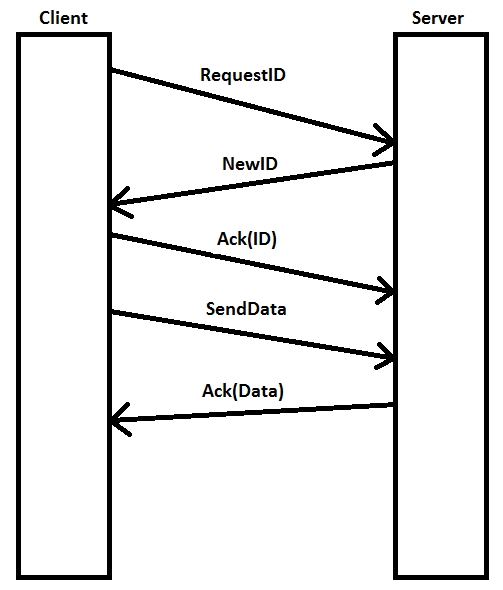
\includegraphics[width=0.4\textwidth]{figures/clientserver.png}
    \caption{Client-server illustration}
    \label{fig:clientserver}
\end{figure}

\figref{fig:clientserver} illustrates how our client-server structure works. The client sends a RequestID command to the server. The server responds with an ID, which is an integer that counts one up after each RequestID.\todo{counts up after what exactly?} The reason the server provides the ID is to prevent clashes, which might occur if the clients generated the IDs. The client sends back an acknowledgement to the server when it has received the ID. If the server does not receive an acknowledgement, it will resend the ID. When the client has received the ID it sends the data to the server that is needed to create a new route, or alter a route, or gives information about the route it is following. The server then sends an acknowledgement that it has received the data. If the client does not receive the acknowledgement, it resends the data and waits repeatedly until it either receives acknowledgement or times out.

The messages that are sent back and forth are converted into bytes. In figure

\section{Data Preprocessing}
The Beijing dataset\todo{Which one? There are two datasets.} consists of timestamped GPS-coordinates. The format of the data is (id, date time, longitude, latitude). The data is raw, so it needs to be map-matched to a road. To perform map-matching, the system calls the TrackMatching webservice\cite{TrackMatching}. This service exposes an API for map-matching to the OpenStreetMap service. Given a dataset of raw GPS-coordinates, it returns a map-matched dataset in JSON format.
\todo{write about how and why map generation}
\todo{write about how and why we design DB and store data in SQL database}
\section{Data analysis}
\todo{How do we analyse the data? What information do we infer (speed, probability of traffic congestion, the design of the cost function to change based on traffic data? How are bayesian networks involved?}
There are 2 processes involved in keeping the data for the map realistic:
\begin{itemize}
	\item Traffic pattern analysis of historical data
	\item Live traffic data analysis
\end{itemize}

The main idea of the traffic pattern analysis is that the data gathered over a given period, at some point will be bulk processed to see if traffic patterns keep the same. Such that the system allways have the best image of the traffic for a particular day, and use these patterns for the best route calculation.

The live traffic data analysis is used check if there are any abnormalities at a given segment, and then being able to propagate this to devices that are going through that segment. Eventually redirecting drivers such that they don't end up at a congested segment, unless nothing else is possible.
\section{Route planning}
\todo{How do we plan the routes? A*/D*, heuristic and cost function for capacity of roads ....}

\chapter{Conclusion}
This project presented an approach for modeling road network and traffic as weighted directed graphs with weight functions as time-based piecewise linear regression models over traffic observations of speed derived from GPS samples.

The piecewise linear regression models was found to have an average predictive accuracy of NUMBER\% of actual observed travel time on routes. This follows from several issues still present in the regression models such as limited data and improvable filtering, and could futher be improved by gathering a more useful dataset where speed is directly measured.

Furthermore the system was found to, in certain cases, be able to find alternative routes avoiding traffic congestion thus potentially provide time-savings for users of the system. By providing such a feature the system can help motorists avoid heavy traffic and be more evenly distributed on the road network.

There are many interesting areas for future work including gathering better GPS data, more accurate map-matching , optimizations in terms of utilizing advanced graph methods such as contraction hierarchies to speed up query time. Furthermore, we find it important to perform field-testing in the future, to get a much better perspective of the accuracy of the system as a whole.

To be able to collect the data needed to predict traffic patterns which our agent needs, we have constructed a client-server architecture, which is described in \secref{chap:clientserver}. The client collects data, speed, time and GPS locations, and sends that to our server where we can store the information.
\printbibliography[heading=bibintoc]
\label{bib:mybiblio}
\appendix
\chapter{Routefinding pseudocode}\label{ch:astar}
\begin{algorithm}
\begin{algorithmic}[1]
\Function{A*}{$Graph$, $Start$, $End$}
  \State create vertex set $Q$ \Comment{Set of unvisited nodes}
  \State
  \ForAll{vertex $v$ \In $Graph$} \Comment{Initialization}
    \State $dist[v] \gets$ INFINITY \Comment{Unknown distance from $Start$}
    \State \Comment{to $v$}
    \State
    \State $heur[v] \gets$ \Call{H}{$v$, $End$} \Comment{Heuristic value from $v$ to $End$}
    \State
    \State $prev[v] \gets$ UNDEFINED \Comment{Previous node in the optimal}
    \State \Comment{path from $Start$}
    \State
    \State add $v$ to $Q$ \Comment{All nodes are initially unvisited}
  \EndFor
  \State
  \State $dist[Start] \gets 0$
  \State
  \While{$Q$ is not empty \AND \Call{OtherDirectionNotDone}{}}
    \State $u \gets$ vertex \In $Q$ with min $dist[u] + heur[u]$
    \State remove $u$ from $Q$
    \State \Call{VisitFromThisDirection}{$u$}
    \State
    \If{$u = End$ \Or \Call{IsVisitedFromOtherDirection}{$u$}}
      \State for this direction: $done \gets$ \True
      \State \Return \Call{ReconstructPath}{$prev$}
    \EndIf
    \State
    \ForAll{neighbours $v$ of $u$} \Comment{where $v$ is still in $Q$}
      \State $alt \gets dist[u]$
      \If{$alt < dist[v]$}
        \State $dist[v] \gets alt$
        \State $prev[v] \gets u$
      \EndIf
    \EndFor
  \EndWhile
  \State \Return empty
\EndFunction
\end{algorithmic}
\caption{A* ready for bidirectional search}
\label{alg:bi_astar}
\end{algorithm}

\begin{algorithm}
\begin{algorithmic}[1]
\Function{BidirectionalSearch}{$Graph$, $Start$, $End$}
  \State $path1 \gets$ run \Call{A*}{$Graph$, $Start$, $End$} concurrent
  \State $path2 \gets$ run \Call{A*}{$Graph$, $End$, $Start$} concurrent
  \State
  \If{$path1 =$ empty}
    \State \Return $path2$
  \Else
    \State \Return $path1$
  \EndIf
\EndFunction
\end{algorithmic}
\caption{Bidirectional search}
\label{alg:bi_search}
\end{algorithm}

\end{document}